\documentclass[journal]{IEEEtran}

\usepackage{ifpdf}

\usepackage{cite}

\ifCLASSINFOpdf
  \usepackage[pdftex]{graphicx}
  % declare the path(s) where your graphic files are
  \graphicspath{{images}}
  % and their extensions so you won't have to specify these with
  % every instance of \includegraphics
  \DeclareGraphicsExtensions{.pdf,.jpeg,.png}
\else
  % or other class option (dvipsone, dvipdf, if not using dvips). graphicx
  % will default to the driver specified in the system graphics.cfg if no
  % driver is specified.
  \usepackage[dvips]{graphicx}
  % declare the path(s) where your graphic files are
  \graphicspath{images}
  % and their extensions so you won't have to specify these with
  % every instance of \includegraphics
  \DeclareGraphicsExtensions{.eps}
\fi

\usepackage[cmex10]{amsmath}
\usepackage{amsfonts}
\usepackage{amssymb}

\usepackage{todonotes}

\usepackage{algorithmic}

\usepackage{array}
\ifCLASSOPTIONcompsoc
  \usepackage[caption=false,font=normalsize,labelfont=sf,textfont=sf]{subfig}
\else
  \usepackage[caption=false,font=footnotesize]{subfig}
\fi

%\usepackage{fixltx2e}

\usepackage{stfloats}

\ifCLASSOPTIONcaptionsoff
  \usepackage[nomarkers]{endfloat}
 \let\MYoriglatexcaption\caption
 \renewcommand{\caption}[2][\relax]{\MYoriglatexcaption[#2]{#2}}
\fi

\usepackage{url}

% correct bad hyphenation here
\hyphenation{op-tical net-works semi-conduc-tor}

\begin{document}

\title{FollowBot Android Application}


\author{Arian~Stolwijk,~\IEEEmembership{4001079}
        and Radu~Florea,~\IEEEmembership{4330358}}% <-this % stops a space

% The paper headers
\markboth{IN4254 - Smart Phone Sensing}%
{}
% make the title area
\maketitle

% As a general rule, do not put math, special symbols or citations
% in the abstract or keywords.
\begin{abstract}

In this report, we present the development process of an Android smartphone application that controls a simple moving robot, such that it always follows the user. A possible application for this robot, with the necessary modifications, is carrying heavy loads over long distances. The robot consists of simple
hardware components, and the computation and sensing is done on the smartphone.
A particle filter is used to estimate the distance and the orientation of the robot with respect to the user.
Measurements of the distance, orientation and heading are done by the phone's
camera, using object tracking. The accelerometer sensor is used to detect
walking activity, with the help of a kNN classifier, and user orientation, used in updating
the particles of the filter. The robot is controlled by a \texttt{IOIO} board,
a simple hardware device that directly follows commands from the phone through
a Bluetooth connection. We found that the particle filter localization
is working well. Measuring the distance with the camera is also functional, however only for short distances.

\end{abstract}

\section{Introduction}

There is an existing assumption that when baby geese come out of their eggs,
they assume that their mother is the first thing they see. Usually this is
true, the baby geese following their mother until they able to fend for
themselves. If a human were to be the first thing the baby geese saw, they
would simply follow the human too.

Using an Android smartphone and a simple robot we can simulate the same effect.
The smartphone acts as the mother (moved by the user) and the robot as the baby
goose. The objective of the robot is to follow the smartphone and, thus, the
person carrying it. This kind of behavior can be used to great effect in moving
very heavy loads over long distances, eliminating the need to constantly
control the robot. Using computational power and sensors of today's
smartphones, specialized and expensive hardware can be eliminated. Instead we
can use a device that many people already have.

We have built an Android smart phone application that controls a remote,
wheeled robot. This robot can move forward and backwards, and turn left or
right. The smartphone sends direction commands to the robot via a Bluetooth
connection.  The robot blindly follows the commands, the Android phone being
the smart component in this setup. For the smarthpone to be smart it should be
able to localize the robot so that it can send appropriate commands to it.

\section{Problem Description}

Localization of the robot is not a trivial task, we need to combine multiple
sensors of the smartphone to achieve an accurate estimate of the location of
the robot. However, in addition to the robot's location, the phone also needs
to know the orientation of the robot, so it can decide whether to send forward,
backwards, left or right commands to the robot.

If the robot cannot be measured entirely, the phone should still track the
location and orientation of the robot. When taking the movements and
rotations of the user and robot into account the robot will continue to be
tracked.

The robot is a simple four wheeled chassis with a \texttt{IOIO} board,
which communicates with Android over Bluetooth. The \texttt{IOIO} board
controls the wheels with a PWM signal with the help of a H-Bridge.

\section{Robot Localization using a Particle Filter}

In \cite{fox1999monte} Monte Carlo Localization (MCL) is used to localize a
mobile robot. MCL is a type of Particle Filter. The advantage of this method is
that it is continuous, i.e.: there is no need for a fine-grained grid, which is
necessary in Markov localization techniques. Compared to Kalman filter-based
techniques, a Particle Filter is multimodal. Finally it is easy to implement
and it allows us to combine different kinds of measurements and movement
models.

The key underlying idea of the particle filter is to represent the belief
of the location as $N$ weighted \emph{particles}. A particle is denoted as
$((x,y,\theta),w)$, the location and orientation of the robot and
the weight of the particle with $\sum_{n=1}^N w_n = 1$.

The particle filter proceeds in three phases. First an \textbf{initial belief
distribution} is created. Here $N$ Particles are randomly distributed around the
origin. This is executed only once.

The next phase is the \textbf{measurement phase}. In this phase measurements
are executed. Measured values are the distance to the robot, the orientation of
the robot and the heading. The heading is the angle between the user and robot:
0 degrees if the robot is exactly in front of the user, $+90$ degrees if the
robot is on the left side of the user and $-90$ degrees if it is on the right
side. Each particle is assigned a weight depending on the measurement, e.g.\
given this measured distance, what is the probability that the distance is
actually the distance of this particle using a Gaussian distribution.

\textbf{Resampling} is done after a measurement. Resampling moves particles
to the location with the highest probability the robot is positioned in. There are multiple
techniques for resampling \cite{douc2005comparison}. We implemented the
simple Multinomial resampling. Figure~\ref{fig:particle-measurement} shows a
3-dimensional plot of the particles after a distance measurement, resampling
and a heading measurement.
%
\begin{figure}[htpb]
 \centering
 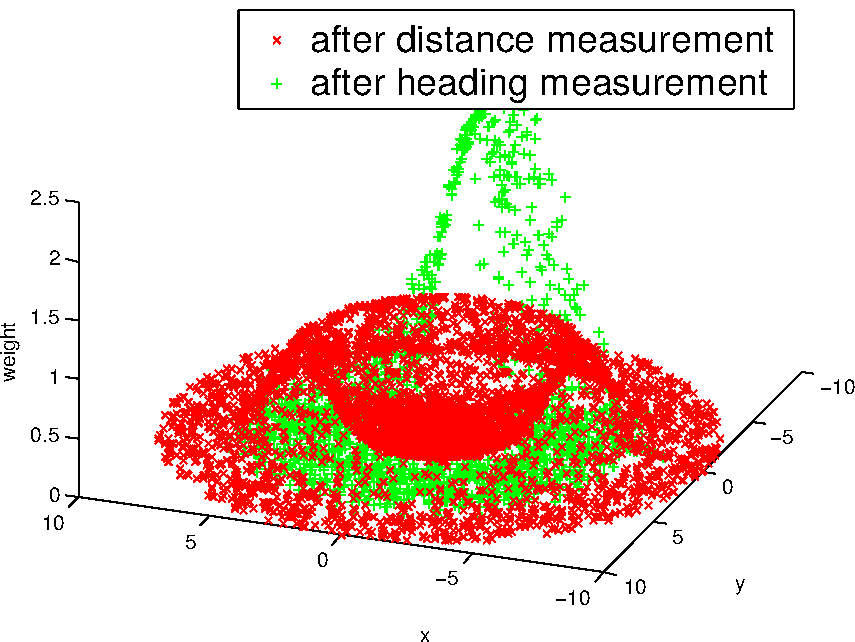
\includegraphics[width=3in]{images/particle-measure.pdf}
 \caption{Weight of particles after a distance measurement. Then the particles
 were resampled, as the green particles have a higher density where the weights
of the red are higher. Finally a heading measurement was executed, which
inreases the weight of the particles in a certain direction.}
 \label{fig:particle-measurement}
\end{figure}
%
\textbf{Movement phase} is where movements are applied to the particles. There
are four types of movement: 1) when the robot is commanded to rotate or 2) move,
or 3) when the user moves or 4) rotates. Figure~\ref{fig:particle-move} shows
how the particles move. A move has a certain uncertainty, which is why the
actual move of a particle is drawn from an probability with the original move
as mean.
%
\begin{figure}[htpb]
 \centering
 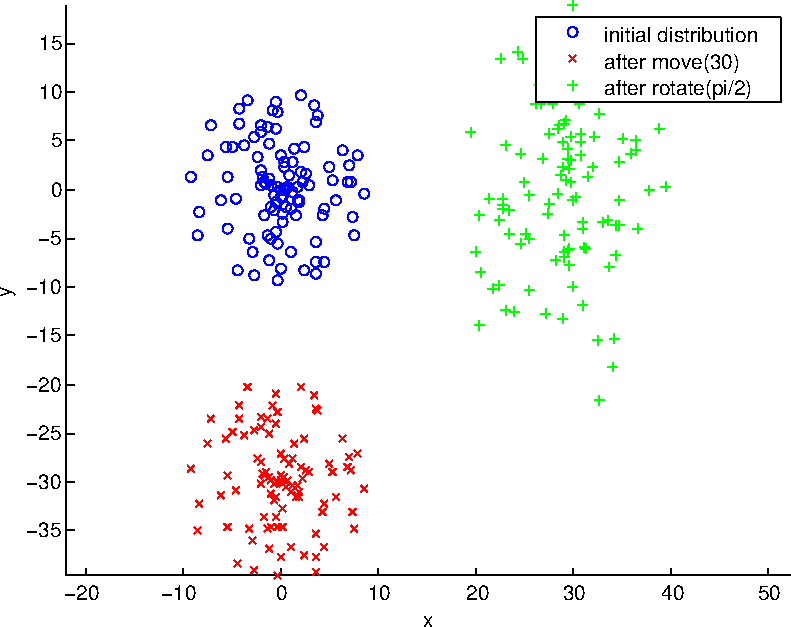
\includegraphics[width=3in]{images/particle-move.pdf}
 \caption{The blue particles is the initial belief, centered around $(0,0)$. Then
 a user movement of $30$ is executed. As the user is always at $(0,0)$, this means
that all particles move around $-30$. Finally rotates $90$ degrees clock-wise,
means the particles will be on the right side of the user. Here the spread,
due to the probability, is clearly visible.}
 \label{fig:particle-move}
\end{figure}

The iterations of measuring, resampling and movements constantly update the
particles. Each type of measurement of movement will be explained in the
following sections.

\section{Distance and Orientation Measurement}

In order to control the robot, the detection of the robot needs to be considered. Furthermore, accurate estimates of the robot's distance and orientation with respect to the user are needed so that a good control can be achieved.

One straightforward solution to the detection problem is to simply make use of
the phone's camera for detecting and tracking three colored spherical objects
(two blue balls and one green ball) that are placed on the top of the robot.

We first start off by converting the colored image from the standard RGB geometry into the HSV (Hue-Saturation-Value) representation. This is done due to the fact that it is much easier to filter out a range of colors in the HSV representation than in the normal RGB case. The HSV color cylinder is presented in figure~\ref{fig:sim}.
%
\begin{figure}[htpb]
 \centering
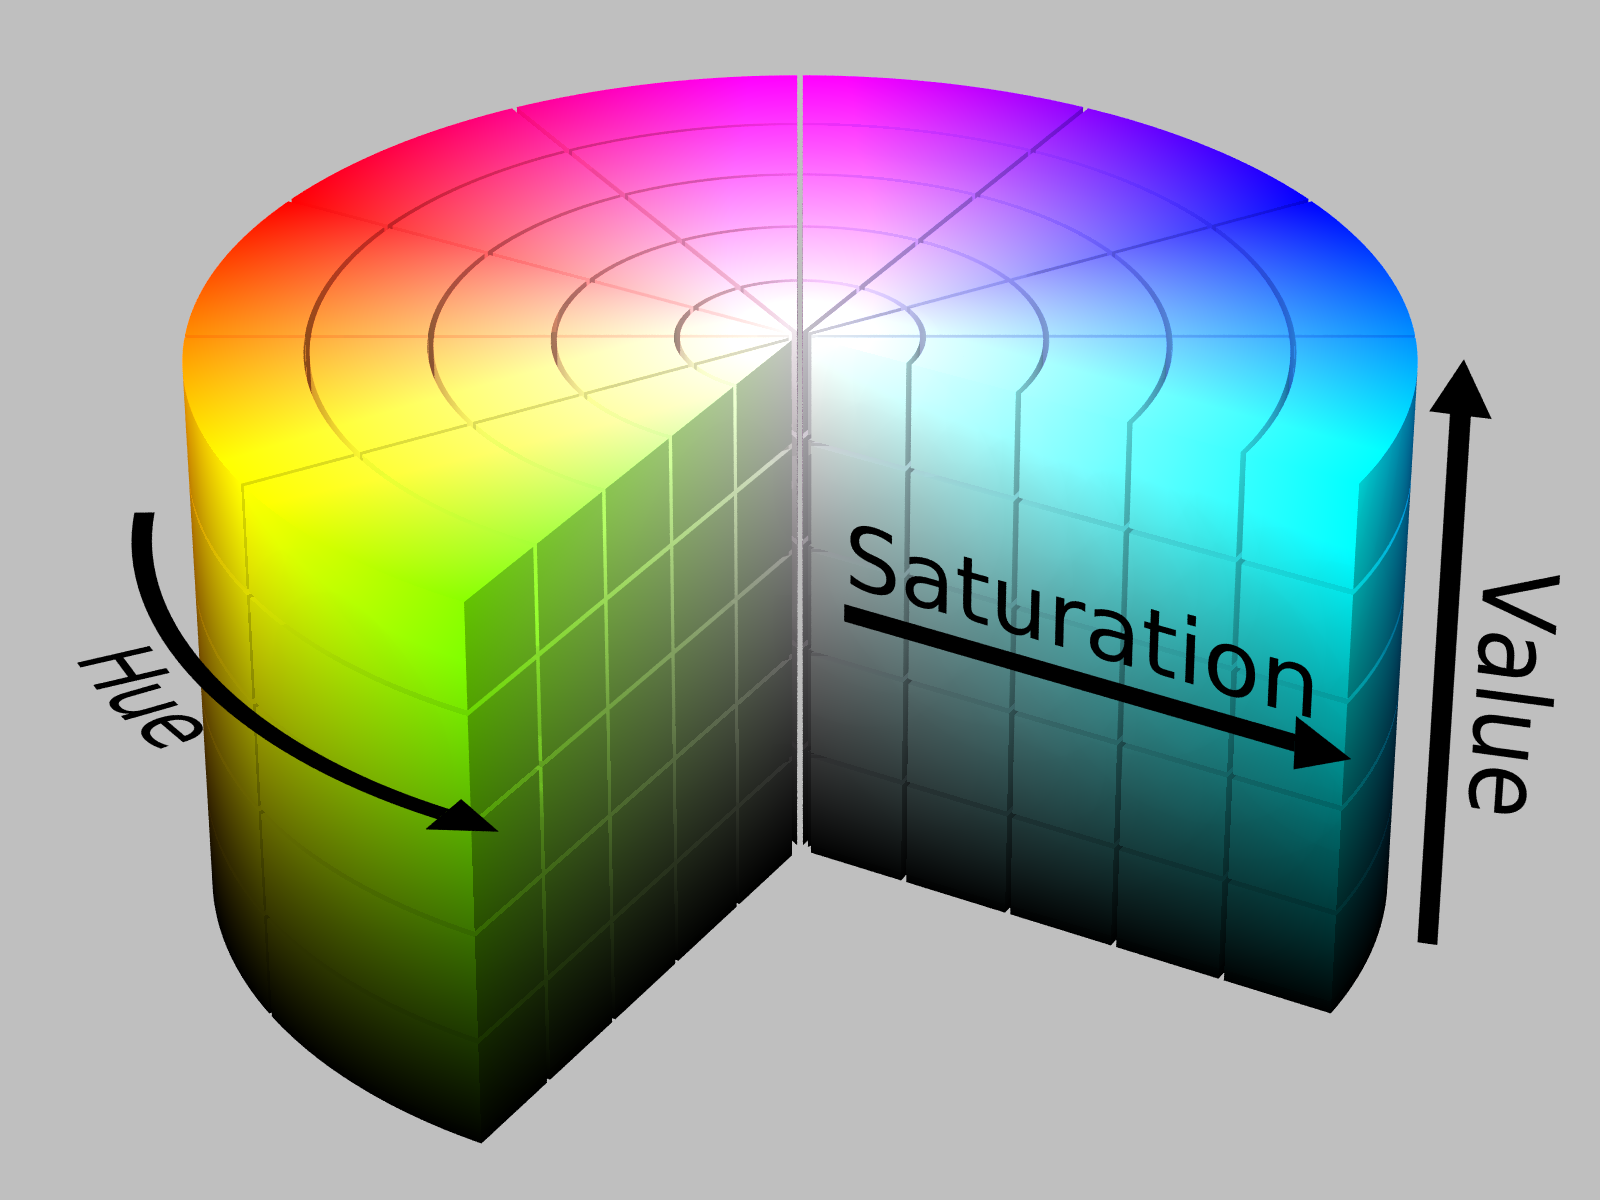
\includegraphics[width=2in]{images/hsv_representation}
\caption{Hue-Saturation-Value color cylinder}
\label{fig:sim}
\end{figure}

Using this representation, the images from the phone's camera can be thresholded based on the colors they contain. Since we are interested in detecting blue and green objects, a set of minimum and maximum bounds has been defined for each of the colors.

The thresholding procedure results in two different images, i.e. one containing data for the color blue and the other one for the color green. These two images are combined into one through the use of an \texttt{OR} operation. This process is shown in Figure \ref{fig:thresh}.
%
\begin{figure}[htpb]
 \centering
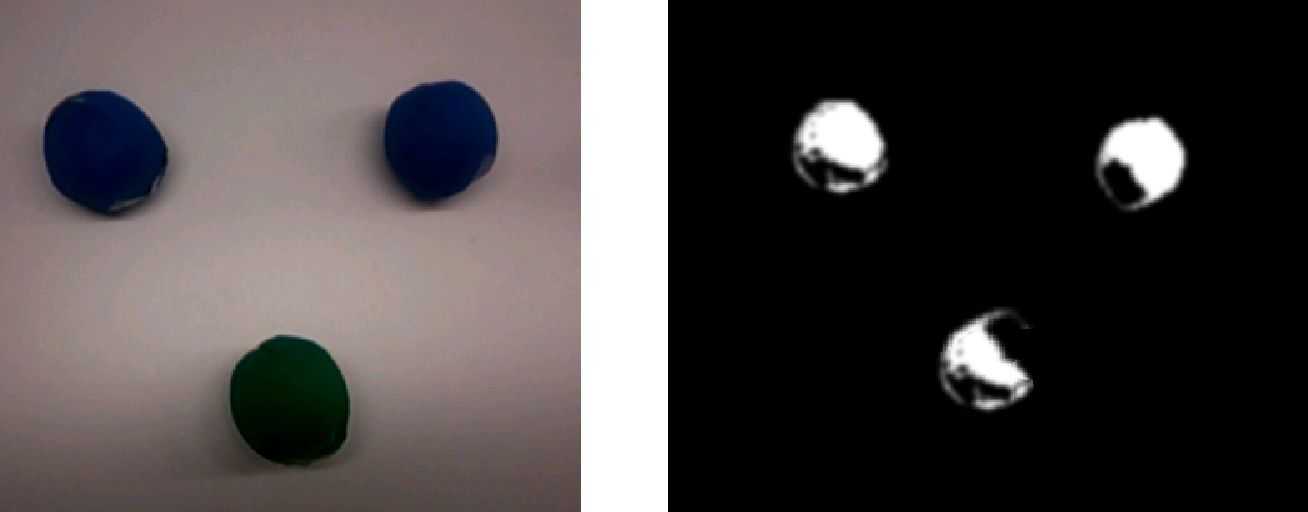
\includegraphics[width=3in]{images/thresholding}
\caption{Image thresholding}
\label{fig:thresh}
\end{figure}

Having the thresholded image obtained, the Circle Hough Transform (CHT) can be applied in order to obtain the three circles present in the image, and track them.

The basic idea underlying the Hough Transform is that, given an image containing a circle described as:
%
\begin{equation}
\left(x-a\right)^2 + \left(y-b\right)^2 = r^2
\end{equation}

where $(a,b)$ are the coordinates of the circle's center and $r$ is its radius, an arbitrary edge point $(x_i, y_i)$ will be transformed into a right circular cone in the $(a,b,r)$ parameter space. If the image points lie in a circle, then the cones will intersect at a single point in $(a,b,r)$, corresponding to the parameters of the circle \cite{yuen1990cht}.

The CHT is also capable of finding circles that are partially hidden, if enough of their boundary is visible. This feature is especially important for the project, since the lighting conditions are not perfect, resulting in parts of the tracking balls that will not be contained in the thresholded image. Such a case is presented in Figure \ref{fig:cht}.
%
\begin{figure}[htpb]
 \centering
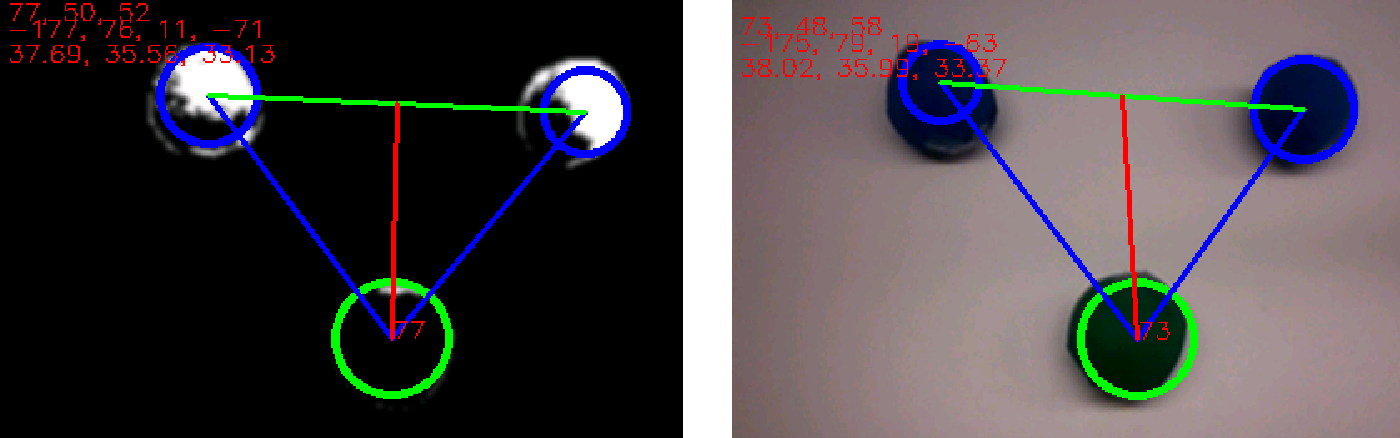
\includegraphics[width=3in]{images/cht_incomplete}
\caption{Circle detection using Hough Transform. Left: Thresholded image, with detected circles. Right: RGB image (in imperfect lighting conditions), with detected circles}
\label{fig:cht}
\end{figure}

As it can be observed, the Hough Transform achieves circle detection even if the image does not contain the entire shape (in this case, almost the entire green ball is missing).

The presented detection method has been implemented, with the help of the \texttt{OpenCV} library, in \texttt{C++}, and it was imported in the Android application through the \texttt{JNI} (Java Native Interface).

\subsection{Distance Estimation}
In order to obtain a decently accurate distance estimation between the robot and the user, and at the same time keep the development costs low, we have explored two techniques for distance estimation, namely: estimating distance with the help of the integrated camera of the Android phone, and distance estimation using the Bluetooth RSS signal.

\subsubsection{Android Phone Camera}
The idea to use the integrated phone camera has been considered due to already having a working spherical object tracking algorithm, thus, we would only have to extend this algorithm to incorporate distance estimation.

From a geometrical point of view, the user to robot distance estimation is presented in Figure \ref{fig:dist_camera}.
%
\begin{figure}[htpb]
 \centering
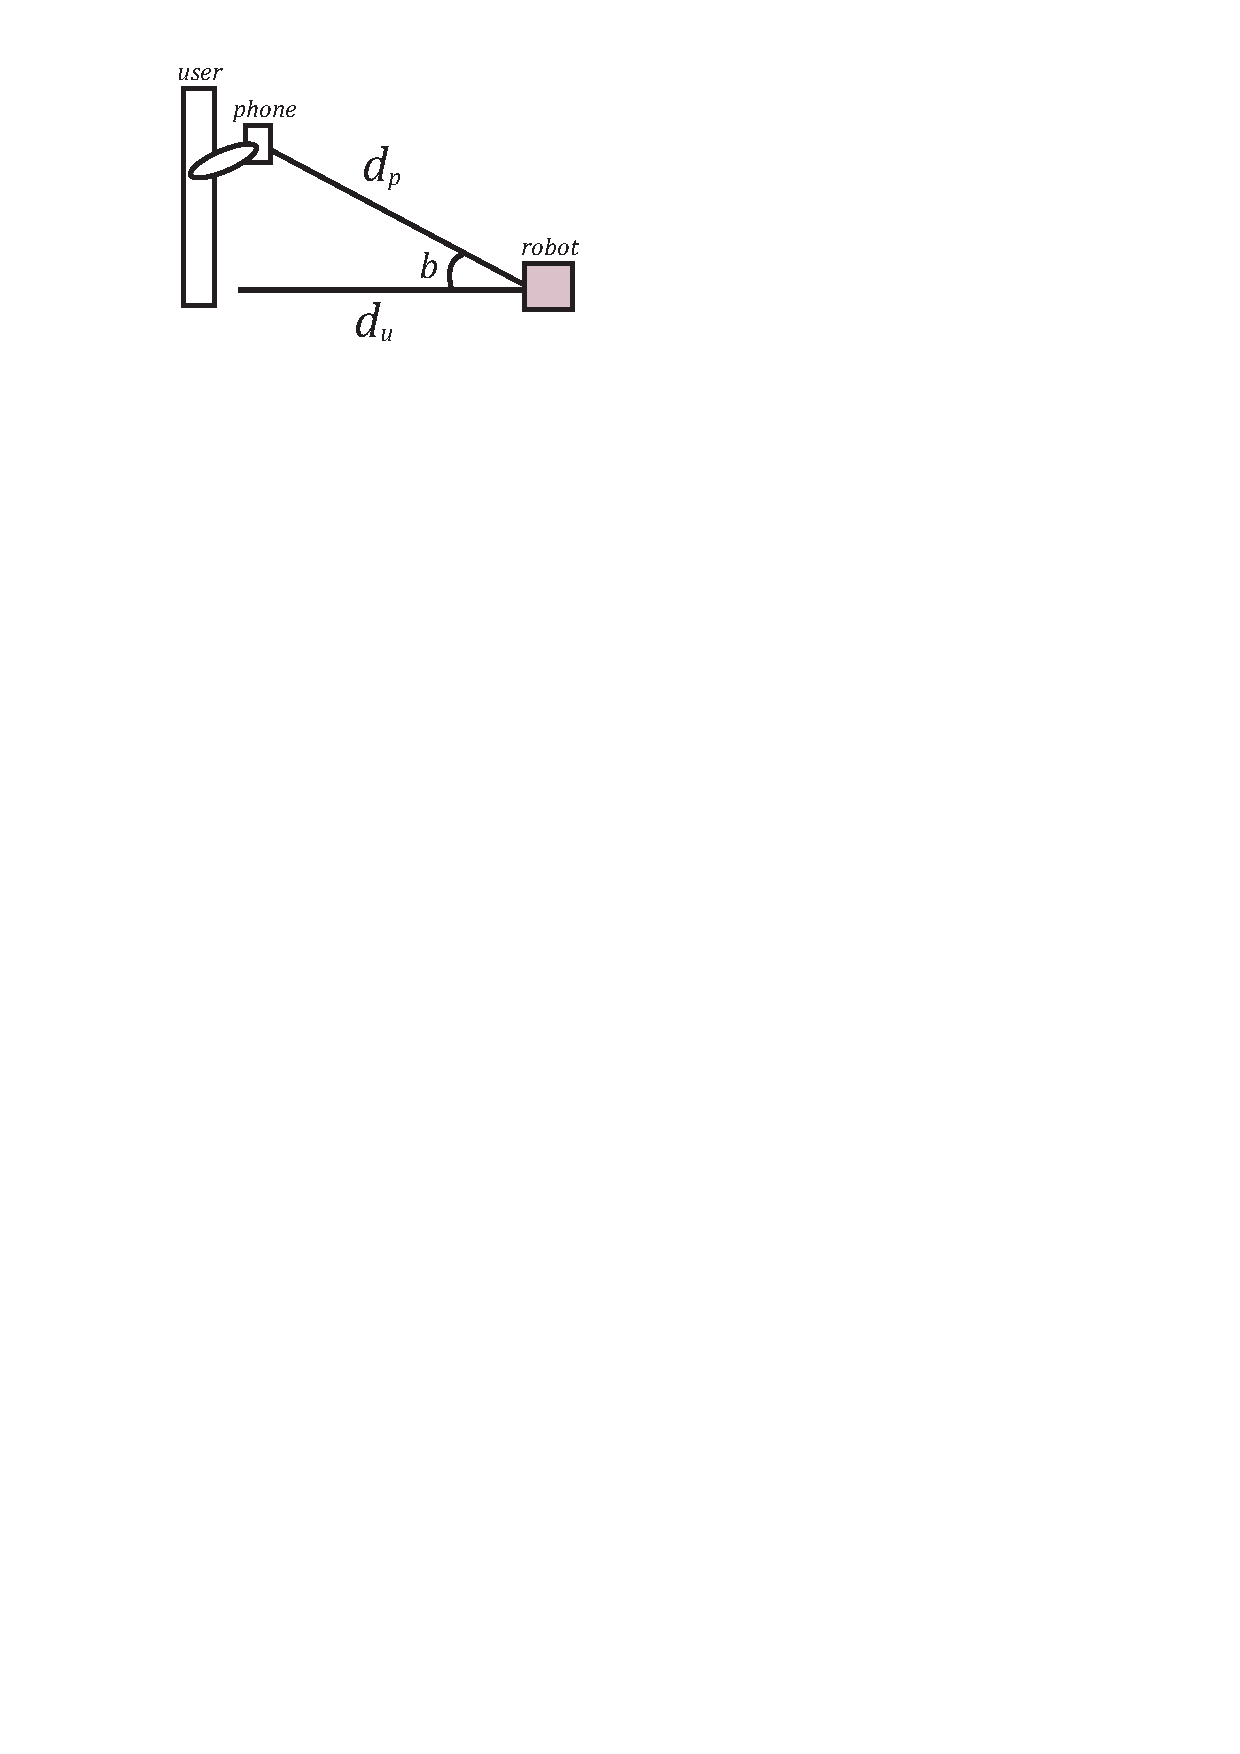
\includegraphics[width=2in]{images/distance_meas}
\caption{Side-view of the distance estimation, using the phone camera. Phone-robot distance is represented by $d_p$, user-robot distance is represented by $d_u$, and the skew angle is represented by $b$}
\label{fig:dist_camera}
\end{figure}

It can be observed that the user-robot distance $d_u$ can be obtained by simply applying the following formula:

\begin{equation}
d_u=d_pcos(b)
\label{eq:dist_estim}
\end{equation}
where the phone-robot distance and the skew angle estimates are given by $d_p$ and $b$, respectively.

In order to obtain an estimate of $d_p$, the radius values of the closest circle (i.e. the largest radius $r_{max}$) has been taken at different distance points, after which a linear interpolation has been applied to these data points, resulting in the following equation for the phone-robot distance estimate
\begin{equation}
d_p=-\frac{24}{31}r_{max}+\frac{1995}{31}
\end{equation}

The skew angle $b$ is estimated in a similar fashion. Considering that the tracking balls are placed in an equilateral triangle shape, a skew angle of $90^{\circ}$ (phone is directly above the robot) corresponds to reading an angle of $60^{\circ}$ from the triangle determined by the tracking objects.

Furthermore, when the skew angle decreases, one of the angles will always increase, while the other two decrease. Thus, for a skew angle of $0^{\circ}$, we know that one of the angles of the triangle, determined by the tracking balls, will be very close to $180^{\circ}$.

Using these two points, and assuming that the relation between the skew angle and the triangle angles is linear, the skew angle $b$ can be defined as
\begin{equation}
b=-\frac{3}{4}\beta_{max}+\frac{540}{4}
\end{equation}
where $\beta_{max}$ is the largest angle of the tracked triangle.

Having the phone-robot distance and the skew angle estimates, the user-robot estimated distance can be computed using Equation \ref{eq:dist_estim}, obtaining an estimate with an error of around $0.2$ meters.

\subsubsection{Bluetooth RSS Signal}
Another method of estimating the distance between the user and the robot is by making use of the RSS signal coming from the Bluetooth connection between the Android phone and the robot.

However, the method has been quickly dismissed due to extremely poor measurement results. Two main problems have been encountered. In the first place, RSS measurements did not have a deterministic sampling time, which is detrimental in the case of robot control applications. Secondly, the measured signal is very noisy, which also leads to an inaccurate distance measurement. The results obtained after repeated measurements of the RSS signal, at different distances is presented in Figure \ref{fig:rss}.
%
\begin{figure}[htpb]
 \centering
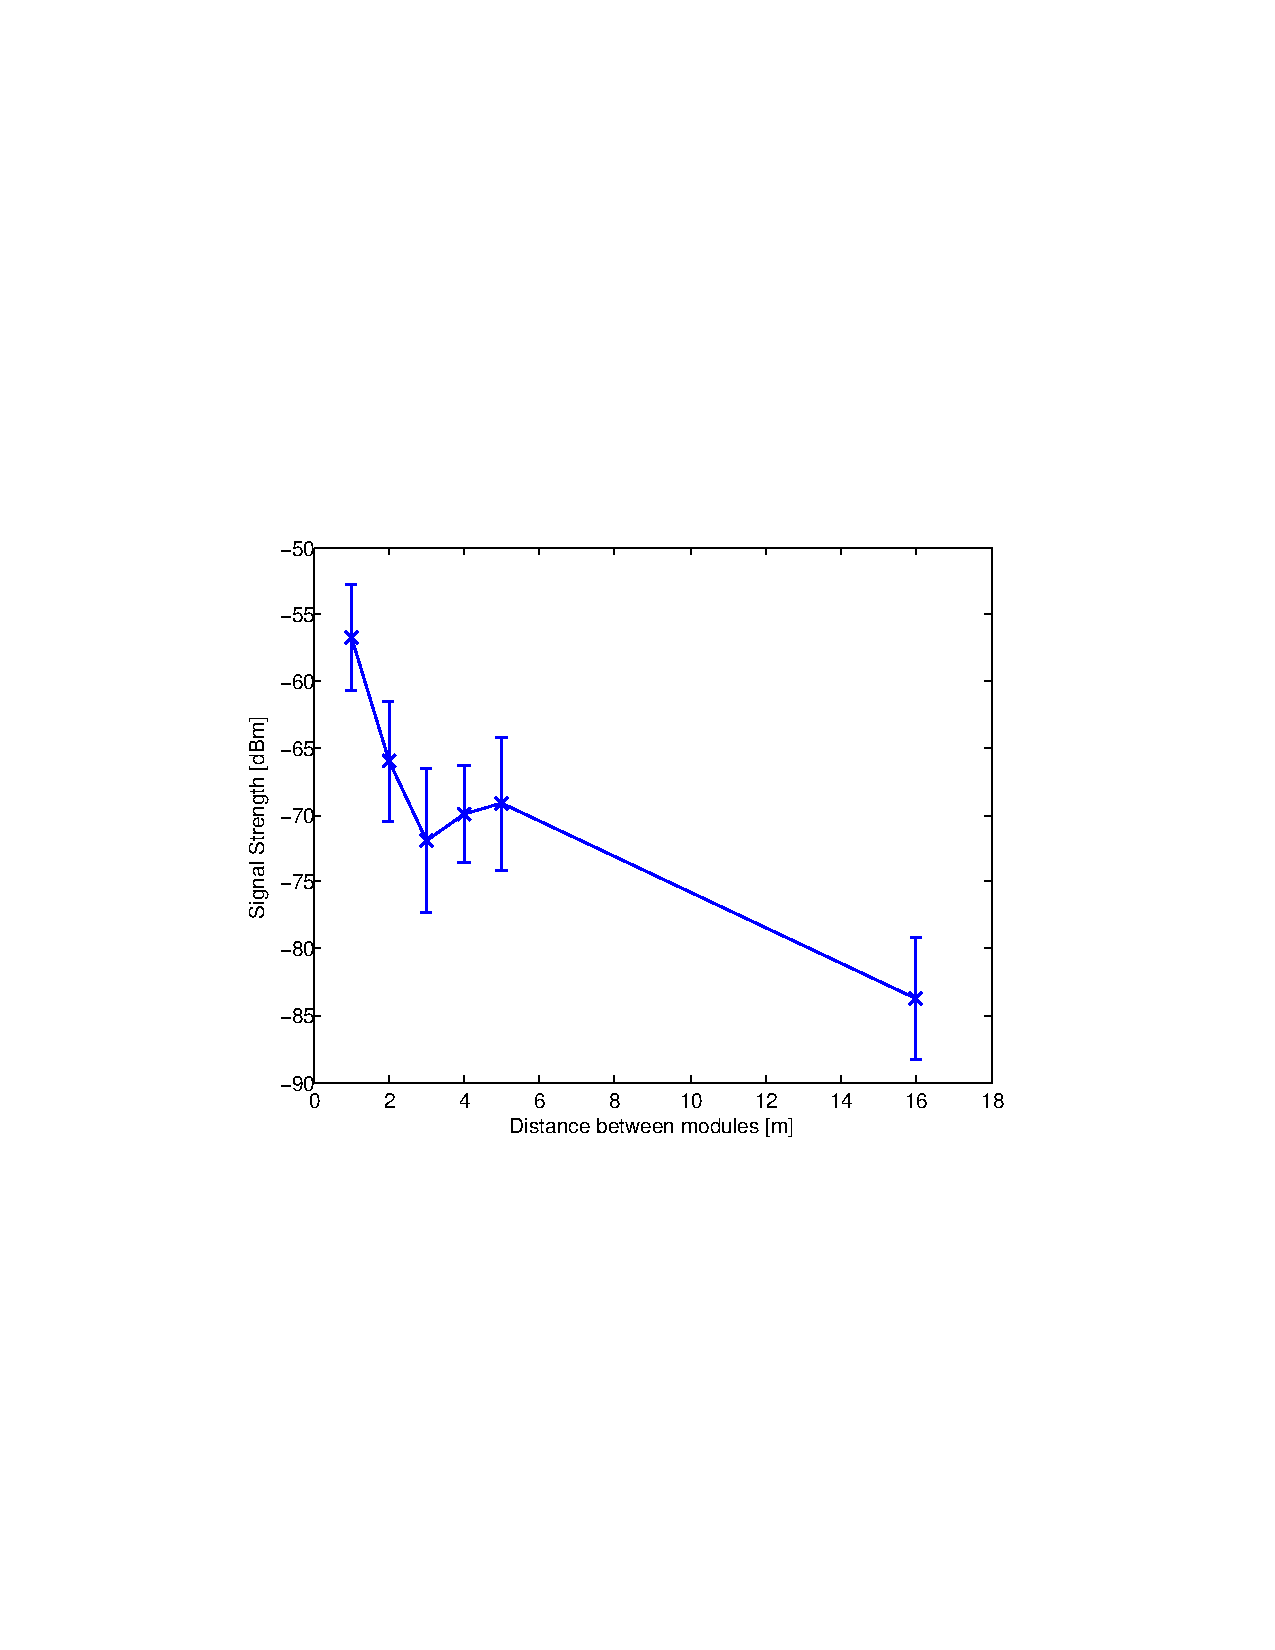
\includegraphics[width=3in]{images/rss_variance}
\caption{Top-view of the orientation estimation, using the phone camera}
\label{fig:rss}
\end{figure}

It can easily be observed that the RSS signal is extremely noisy and would not yield good results in estimating relatively short distances.

Having implemented and tested both distance estimation techniques, the decision to integrate the camera distance estimations in the particle filter algorithm is implicit.

\subsection{Orientation Estimation}

Another aspect that needs to be accounted for when running the particle filter algorithm, is the robot's orientation with respect to the user. A schematic is presented in Figure \ref{fig:orient_camera}, where $a$ is the robot's orientation with respect to the user.
%
\begin{figure}[htpb]
 \centering
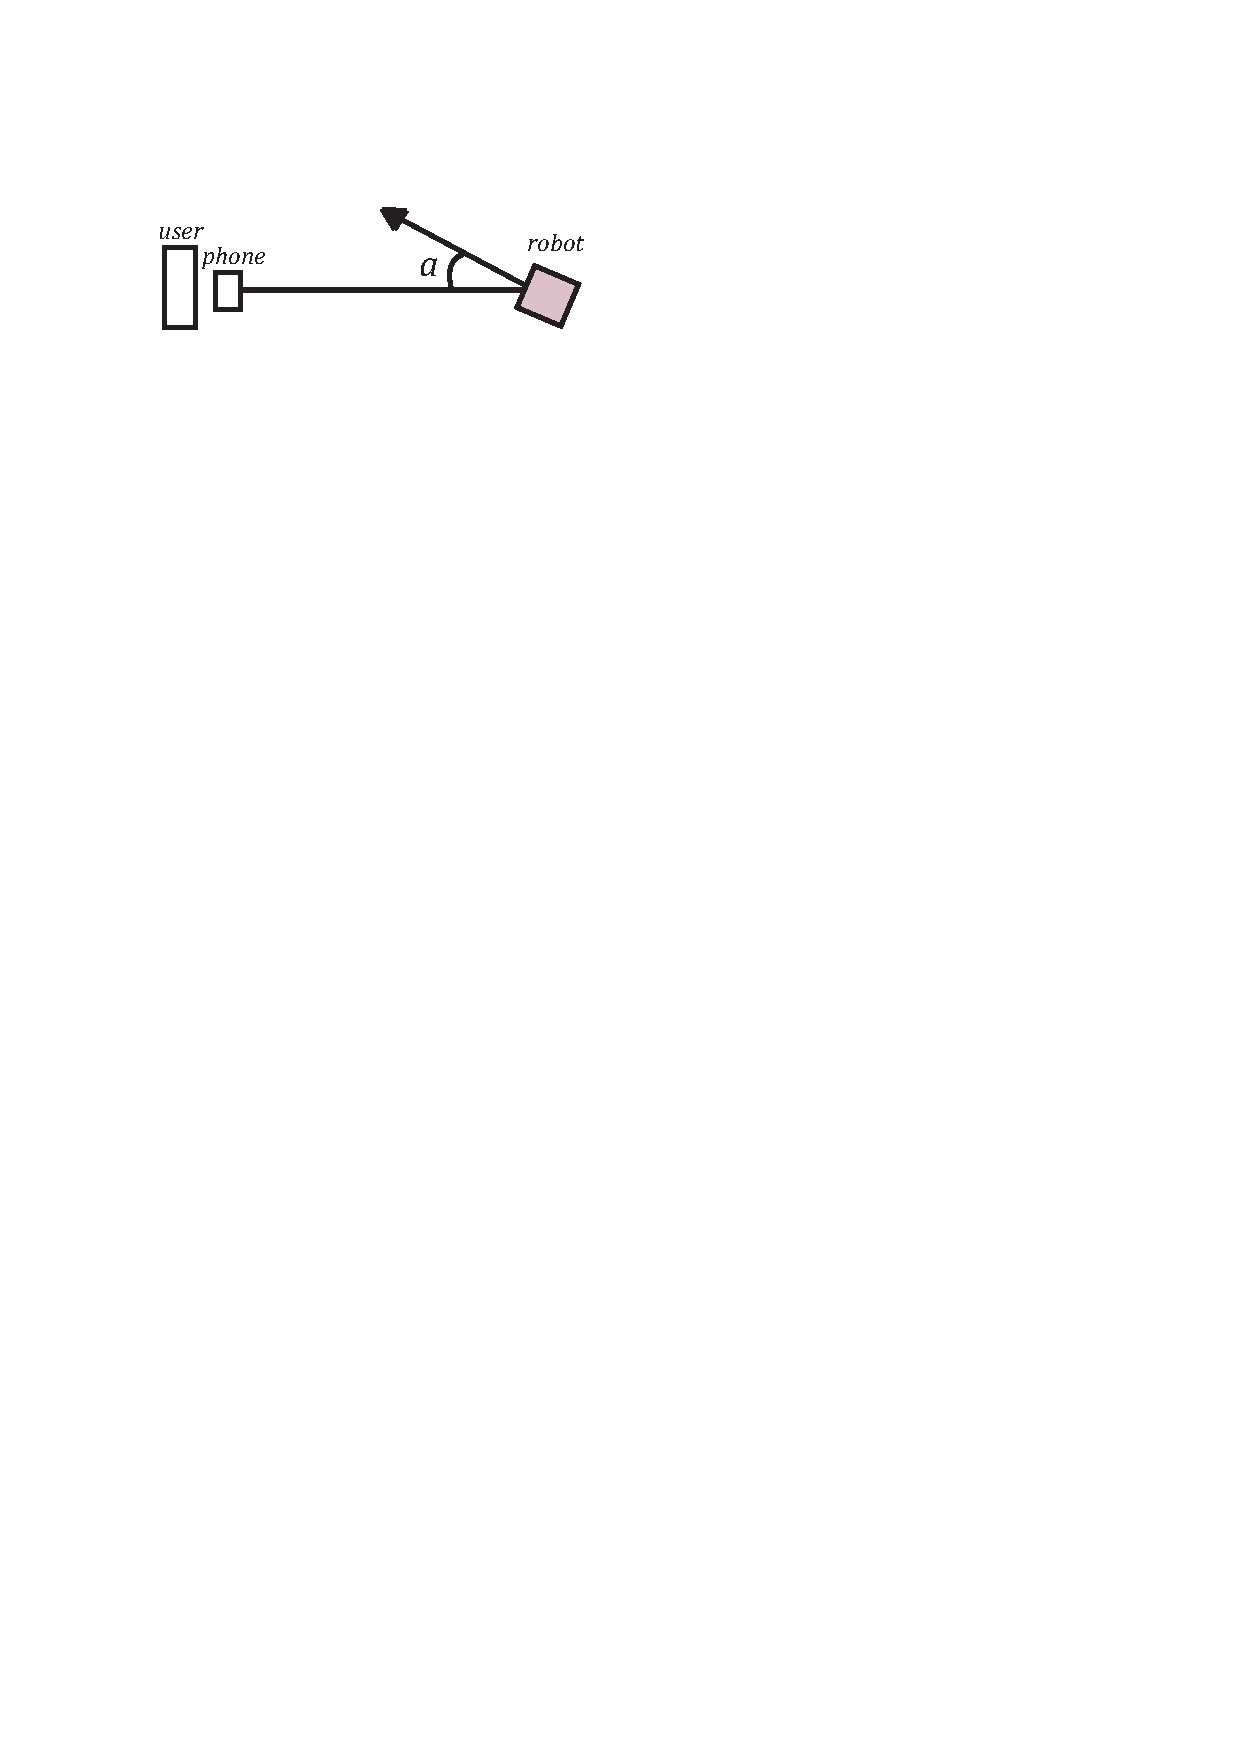
\includegraphics[width=2in]{images/orientation_meas}
\caption{Top-view of the orientation estimation, using the phone camera}
\label{fig:orient_camera}
\end{figure}

Assuming that the robot will always have an orientation between $(-\pi, \pi]$, analytical geometry can be used to determine the angle formed by the camera's X-axis and the line connecting the two blue balls. This corresponds exactly to computing the slope of a line, determined by two points:

\begin{equation}
a=\frac{y_2-y_1}{x_2-x_1}
\end{equation}

In order to obtain an estimated angle between $(-\pi, \pi]$, the \texttt{atan2} function is used when implementing the formula in \texttt{C++}. The obtained estimate has an error of around $0.05$ radians.

\subsection{User Heading Measurement}
Having detected the robot, the user's heading with respect to the robot is set to zero. This is done in order for the assumption that the robot -- when detected by the camera -- is always in front of the user to hold.

\section{User Movement through Activity Monitoring}

When the user moves the particle filter should be updated. To know when the
user is moving can be done with Activity Monitoring. Activity monitoring uses
sensors to identify what the user is doing, for example standing, walking,
cycling or running. Using the activity a speed can be associated to update the
particles in the particle filter. For our application differentiating between
standing still and walking will be enough. \cite{ravi2005activity} showed
different classification techniques using an accelerometer. Features they use
are the mean, standard deviation, energy, correlation and periodicity.  For the
two different activities we expected that the energy and the periodicity to
be enough. \cite{ravi2005activity} also compares different classifiers.
Although the $k$-Nearest-Neighbors is not the best, it is really close to the
best classifier. This combined with that it is relatively easy to implement
makes the kNN classifier a good choice.

The accelerometer stores the $x$, $y$ and $z$ acceleration in a fixed size
data structure with a size of 128 values. This corresponds with a window size
of approximately $1.3$ seconds.

The feature vector $\mathbf{v} = [ZC(\vec x) / t, P(\vec x)/ n]^\intercal$,
where $t$ is the time between the first and last points, and $ZC(\vec x)$ and
$P(\vec x)$ are calculated by:

\begin{equation}
  s(x,y) = \left\{
    \begin{array}{l l}
      1 & \quad \text{if~} x \cdot y < 0 \\
      0 & \quad \text{if~} x \cdot y >= 0
  \end{array} \right.
\end{equation}

\begin{equation}
  ZC(\vec x) = \sum^{n-1}_{i=0} s(x_i, x_{i+1})
\end{equation}

\begin{equation}
  P = \sum^{n}_{i=0} x_i^2
\end{equation}

The kNN classifier consists out of two phases: a learning phase, where feature
vectors with a known class (activity in this case) are stored. This results in
in a plot like figure~\ref{fig:knn-data}.
%
\begin{figure}[htpb]
 \centering
  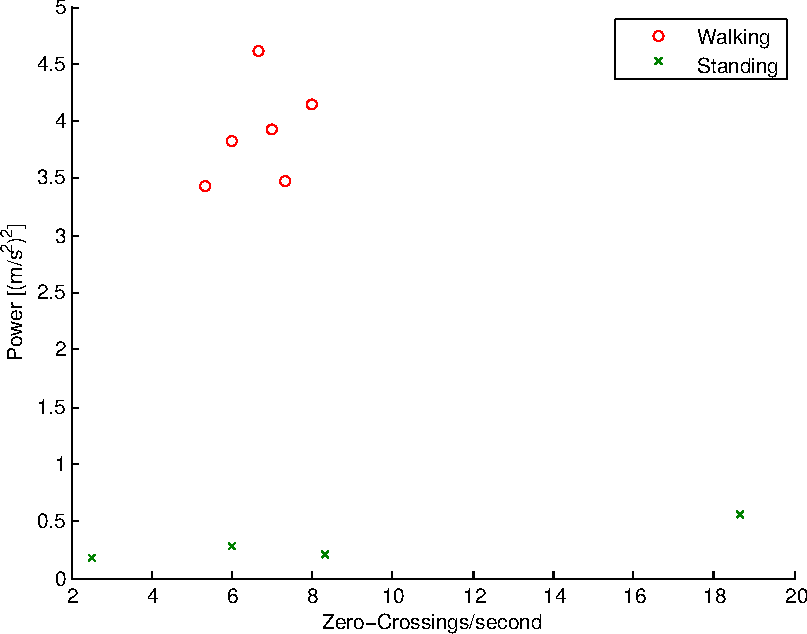
\includegraphics[width=3in]{images/knn-data.pdf}
  \caption{kNN Learning data}
  \label{fig:knn-data}
\end{figure}

The second phase is the classification phase. A newly measured feature vector
is compared with the learning data. By selecting the $n$ nearest neighbors,
counting how many points each class has and finally selecting the class with
the highest count.

The distance between a measurement and the learning data is calculated by the
Euclidean distance. Because the elements from the feature vectors have
different units, we cannot simply apply $\sqrt{ x^2+y^2 }$. Instead we need to
scale the values and make them dimensionless. We do this by finding the minimum
and maximum values of each $i$th element of all vectors, and scale the elements
between $0$ and $1$. The measured value is scaled so eventually we can
calculate the distance.

We have found that 10 learning data points, $n=3$, a window size of $1.3$s
and the chosen features give accurate results classifying walking and standing.

\section{User Orientation}
The user rotation is measured using the accelerometer (gravity) and the
magnetic field sensor of the smartphone. Android has convenient methods to get
the user orientation. The two types of sensors can be combined in the
\texttt{SensorManager.getRotationMatrix} function which fills a rotation
matrix. From this rotation matrix the orientation can be extracted using the
\texttt{SensorManager.getOrientation} function. This returns the yaw, pitch
and roll, though we are only interested in the yaw. Each time we want to update
the particle filter we can take the difference and feed that into the particle
filter.

\section{Robot Movement Model}
The particle filter contains a robot movement model, in order to be able to apply the same type of movement (or at least a relatively good estimate) to all particles whenever the real robot moves.

\subsection{Robot Displacement Model}
The robot's displacement model has been simplified as much as possible, i.e.: it has been assumed that the robot only performs a forward translational movement, along its direction, at a constant velocity, thus, allowing the computation of its displacement at every sample instant.

Based on the characteristics of the physical robot, we have estimated a displacement velocity of around $0.1$ meters every $0.25$ seconds.

\subsection{Robot Rotation Model}
The robot rotation is similar to the robot movement model in the sense that it is assumed that the robot rotates with a constant angular velocity. Again, based on the physical characteristics of the robot, we have estimated an angular velocity of around $0.05$ radians every $0.25$ seconds.

\section{Robot Control}
By combining all the previously described components into the particle filter, robot distance and orientation estimates, with respect to the user, are obtained even when the filter does not receive measurements from the camera. This allows the development of one \texttt{ON-OFF} controller used to keep the robot's orientation around $0$ radians, and a second one used to maintain a certain distance between the robot and the user.

\section{Experimental Setup and Used Libraries}

The project's experimental setup consists of a small-scale, 4-wheeled, $206\mathrm{x}200\mathrm{x}62\ mm$ robotic chassis, controlled by a \texttt{IOIO} board with the help of an \texttt{L298N} H-bridge module. The \texttt{IOIO} board communicates with the Android smart phone through a Bluetooth connection, achieved with the help of the \texttt{LogiLink} Class 1 Bluetooth dongle. On top of the setup, the three, previously mentioned, colored balls are placed. The robot chassis is presented in Figure \ref{fig:robot}.
%
\begin{figure}[htpb]
 \centering
  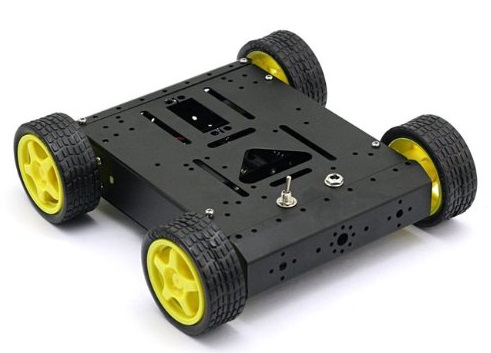
\includegraphics[width=1.5in]{images/robot}
  \caption{Robot chassis used for the project. It has four independent DC motors, controlling each wheel separately.}
  \label{fig:robot}
\end{figure}

The smart phones used in developing the Android application are the following: HTC Desire V, running Android 4.0.3 (Ice-Cream Sandwich) and Sony Xperia SP, running Android 4.3 (Jelly Bean).

The libraries used for developing the different modules of the application, excluding the \texttt{Android API}, were: the \texttt{OpenCV} libraries for computer vision and image processing, used in detecting the robot, and estimating its distance and orientation with respect to the user; the \texttt{IOIO API} was used in order to communicate with the \texttt{IOIO} board and to use the board's features. Also, the \texttt{Java} classes, used for the density and quantile computations (contained in the \texttt{nl.tudelft.followbot.math} package), are part of the \texttt{PAL 1.4} phylogenetic analysis library.

\section{Future Work}

During the development of the application we made several assumptions. In
hindsight there are several spots improvements can be made.

The distance estimation of the robot using the camera and colored balls worked
very well, for smaller distances. When the distance increased, for roughly
more than 1.5 meters, the object tracking did not recognize the balls perfectly
anymore, or found other objects, e.g.\ a computer screen, instead of the balls.
When using better object recognition, using a more unique pattern, like a
chessboard pattern, the object tracking and distance measurements can be improved.

Activity Monitoring works really well classifying standing or walking. However
there is a big assumption that the walking speed is constant. Linking the
periodicity, the number of zero crossings, or frequency using a Fourier
Transform, to the walking speed this can be improved. Adding more classes,
like running, can help to increase the user movement estimation.

\section{Conclusion}

We have built a smartphone application for Android to control a driving robot
which follows the user. To control the distance and orientation are estimated
with an particle filer. The filter has in total seven inputs: three types of
measurements: distance, heading and robot orientation measurements with the
camera, user movement through activity monitoring with a kNN filter using
the accelerometer, user movement using the magnetic and gravity sensors. Robot
movement and rotation for the particle filter are the same values used to
control the robot.

Using the \texttt{IOIO} board and library we can control the robot: make it
move forward and make it rotate.

By connecting the localization and the robot control we will make the robot
follow us.


\bibliographystyle{IEEEtran}
\bibliography{report}

\end{document}
